% paper/manuscript/shellform_cas.tex
% ShellForm manuscript for Computers & Structures (Elsevier, elsarticle).
% Assembled 14 Nov 2026 (check window, day 2) from paper/10-15 drafts.
% Every number has a row in paper/numbers.md (freeze tag freeze-2026-11-09,
% ShellBench v0.3.0; verification rows from main after the 14 Nov merge).
% Tables are built by scripts/day18_manuscript_tables.py from paper/tables/.
% Build: latexmk -pdf shellform_cas.tex   (see paper/manuscript/README.md)
%
% Review marks: \chk = a source the author must still open ([check]);
% \jud = Claude's judgement the author accepts or cuts ([J]);
% \unk = a value still missing ([?]). Set \reviewmarksfalse to hide them.

\documentclass[preprint,12pt]{elsarticle}

\usepackage[T1]{fontenc}
\usepackage[utf8]{inputenc}
\usepackage{lmodern}
\usepackage{amsmath,amssymb}
\usepackage{graphicx}
\usepackage{booktabs}
\usepackage{array}
\usepackage{xcolor}
\usepackage{lineno}
\usepackage{rotating}
\usepackage[hidelinks]{hyperref}
\usepackage{url}

\biboptions{numbers,sort&compress}
\journal{Computers \& Structures}

\newif\ifreviewmarks
\reviewmarkstrue
\definecolor{markcol}{HTML}{B4462B}
\ifreviewmarks
  \newcommand{\chk}{\textsuperscript{\textcolor{markcol}{\sffamily\scriptsize[check]}}}
  \newcommand{\jud}{\textsuperscript{\textcolor{markcol}{\sffamily\scriptsize[J]}}}
  \newcommand{\unk}{\textcolor{markcol}{\sffamily\small[?]}}
\else
  \newcommand{\chk}{}
  \newcommand{\jud}{}
  \newcommand{\unk}{}
\fi

\graphicspath{{../../figures/}}
\newcommand{\figwidth}{\textwidth}

\begin{document}

\begin{frontmatter}

\title{Does seismic-aware form-finding lower the embodied carbon of reinforced concrete shells? A pre-registered comparison of 168 sized designs\jud}

\author{Syed Nafiz Reja Hasib\corref{cor1}}
\ead{syednafiz2811@gmail.com}
\cortext[cor1]{Corresponding author.}
\address{Affiliation \unk}

\begin{abstract}
Seismic-aware form-finding has been developed for shells and arches whose material carries little or no tension. For reinforced concrete shells it is not known whether such a form lowers embodied carbon once the shell is sized to code checks. We compare gravity-only form-finding with a seismic-aware extension of Michiels and Adriaenssens' method: a three-dimensional force density network with four directions of shaking. All 168 designs, square shells of 10 and 20~m on corner or edge supports at three rise-to-span ratios and plateau spectral accelerations from 0 to 0.6~g, are sized to the same checks: a linear buckling factor of at least 5, deflection within span/300, a 50~mm minimum thickness and the minimum steel ratio. Cradle-to-gate (A1--A3) carbon uses GB/T 51366-2019 factors with a $\pm$25\,\% band. The decision rule and sensitivity runs were pre-registered. In 79 of 84 comparisons the two strategies differ by less than 5\,\% (no meaningful difference). The other 5 are one 5~mm thickness step and disappear in every sensitivity run. The cause is the governing checks. Linear buckling sets the thickness of all 84 corner-supported shells, the 50~mm minimum sets all 84 edge-supported shells, and the minimum ratio sets the steel. None responds to the seismic level, so the gravity form carries 1.000--1.004 times its zero-seismic carbon up to 0.6~g. The buckling factor matters far more: at 3 and 8, the carbon of the gravity-form corner shells is 0.736--0.812 and 1.220--1.295 of the baseline. Code and results are open.
\end{abstract}

\begin{keyword}
form-finding \sep force density method \sep reinforced concrete shells \sep embodied carbon \sep seismic design \sep linear buckling \sep pre-registration
\end{keyword}

\end{frontmatter}

\linenumbers
\setlength{\emergencystretch}{1.5em}

%% ---------------------------------------------------------------------
\section{Introduction}\label{sec:intro}

Thin concrete shells carry load mainly by membrane action, so they need far less material than members that carry it in bending. Recent work has turned this into measured carbon savings. A thin-shell floor was designed, built and tested as a low-carbon alternative to a flat slab \cite{Hawkins2019}. Compared with reinforced concrete flat slabs, shell floors may cut cradle-to-gate embodied carbon by up to 65\,\% \cite{Jayasinghe2022}\chk, and a segmented shell floor prototype by about 50\,\% \cite{Oval2023}\chk. Form-finding with the force density method, combined with finite element checks and reinforcement design, is now used to search directly for low-carbon reinforced concrete shells \cite{Leonardi2026}\chk.

These savings were found for gravity loads. In a seismic region a designer must also carry lateral load, and the form that is efficient under gravity is not the form that is efficient under lateral load\jud. Michiels and Adriaenssens addressed this for masonry: they added lateral load to form-finding, so that a compression-only load path exists under combined gravity and seismic load \cite{Michiels2017IASS,Michiels2018CS}\chk. Later work extended the idea to corrugated shells with pushover validation \cite{Michiels2019}, to iso-resistant compression-only shells \cite{Olivieri2025} and to arches, where a seismically form-found shape saved 10--50\,\% of material against a constant-thickness arch \cite{MalagaChuquitaype2022}\chk. In all of these the material has little or no tensile capacity, so the form must keep the thrust inside the section.

Reinforced concrete shells do not need a compression-only form, because reinforcement can carry tension. Their seismic behaviour has been studied mainly on gravity forms. Small and midsized concrete roof shells (spans below 30~m) were found to stay elastic under earthquake excitation, because their high stiffness and low mass place their natural frequencies far above the dominant frequencies of ground motion \cite{Hammood2023}\chk. Nonlinear analyses of force-density reinforced concrete shells under synthetic accelerograms show controlled damage, and show that geometric imperfections reduce their ultimate capacity by 22--45\,\% \cite{PerezVega2026}\chk; fragility analysis of a free-form shell places its damage near the supports \cite{CaycedoGarcia2025}\chk. Michiels and Adriaenssens also identified the design parameters that govern the earthquake resistance of reinforced concrete shells \cite{Michiels2017ES}\chk. These studies analyse a given form. They do not ask whether a form found for seismic load would lower the material, and so the carbon, of a reinforced concrete shell that meets the same code checks.

So two lines of work have not met\jud. Seismic-aware form-finding has been developed where the form must do all the work, in masonry and unreinforced materials. The carbon of reinforced concrete shells has been studied for gravity forms. We found no study that reports what seismic-aware form-finding costs or saves in embodied carbon when reinforced concrete shells are sized to code checks (search protocol in the supplementary material, Section~S1). A designer in a seismic region therefore cannot tell whether a seismic-aware form is worth the extra design effort, or whether a gravity form, checked and sized for the seismic case, already gives the lower-carbon roof\jud.

This paper answers that question for square reinforced concrete roof shells of 10 and 20~m on corner or edge supports, at three rise-to-span ratios and seven plateau spectral accelerations from 0 to 0.6~g. We compare two strategies on equal terms: gravity-only form-finding, and seismic-aware form-finding that extends the method of Michiels and Adriaenssens to a three-dimensional force density network and four directions of shaking. Every one of the 168 designs is sized to the same code checks, and its A1--A3 carbon is computed with GB/T 51366-2019 factors \cite{GBT51366} and a $\pm$25\,\% band. The comparison rule, thresholds and sensitivity runs were pre-registered before any design was run.

The study makes three contributions. First, an open and verified pipeline: a three-dimensional force density solver with a four-direction lateral-load envelope, verified by five pre-registered tests (S1--S5), cross-checked against the finite element wrapper of our earlier benchmark, ShellBench \cite{ShellBench}, and checked again after the freeze against a closed-form buckling load, mesh refinement and the equilibrium residual. Every result is released with the code. Second, a pre-registered comparison of the two strategies over 168 sized designs, with the result and its mechanism: which code check sets the thickness and steel, and why the seismic level does not reach the carbon. Third, a measure of what does move carbon in these shells, the support condition and the buckling factor, which no code fixes. Section~\ref{sec:methods} describes the method, Section~\ref{sec:results} the results, and Section~\ref{sec:discussion} discusses them, their limits, and where we expect the result to change.

%% ---------------------------------------------------------------------
\section{Methods}\label{sec:methods}

\subsection{Overview and pre-registration}

We compare two ways of finding the form of a reinforced concrete shell: a gravity-only form and a seismic-aware form. Each form is sized to the same code checks, and we measure its embodied carbon. The question is whether the seismic-aware form changes the carbon of a shell that meets those checks, and by how much.

The study was pre-registered on 30 October 2026, before any design was run. The pre-registration fixed the design space, the loads, the checks, the carbon basis, the decision rules and the validation tests with their tolerances. Every later change is a dated amendment that says why it was made and whether it was written before or after the results it affects. The amendments are summarised in the supplementary material (Section~S3) and given in full in the repository.

All results come from one run of the frozen code (git tag \texttt{freeze-2026-11-09}). The code is pinned to ShellBench v0.3.0, our earlier validated model, from which every material value, load, code factor and carbon factor is read in place \cite{ShellBench}. ShellForm copies no ShellBench value. The code, results and figures are archived as ShellForm v0.1.0 \cite{ShellForm}.

\subsection{Design space}

The design space has 168 sized designs (Table~\ref{tab:design}). Each one is a square-plan shell with a span $L$ of 10~m or 20~m, supported either at its four corners or along its four edges. The rise-to-span ratio $f/L$ is 0.10, 0.15 or 0.20. Each shell is found by one of the two strategies and sized for one of seven plateau spectral accelerations, $S_a = 0$ to 0.6~g in steps of 0.1~g.

The corner-supported shells need one more choice. With equal force densities everywhere, their free edges pulled in by $0.24L$ and the shell kept only 38\,\% of its plan area, which is not a usable roof. We therefore set the force density of the boundary edges so that each free edge is drawn in by $0.10L$ at mid-edge. This value is a judgement; it was fixed on one shell before the design space was run, and it is the same for every span and rise.

\begin{table}[!htbp]
\centering
\caption{Design space. Each design is sized separately and has one uniform thickness. Corner-supported free edges are drawn in by $0.10L$ at mid-edge.}
\label{tab:design}
\small
\begin{tabular}{ll}
\toprule
Variable & Levels \\
\midrule
Plan & square \\
Span L [m] & 10, 20 \\
Supports & four corners; four continuous edges \\
Rise-to-span ratio [-] & 0.10, 0.15, 0.20 \\
Form-finding strategy & gravity-only; seismic-aware \\
Plateau spectral acceleration Sa [g] & 0.0, 0.1, 0.2, 0.3, 0.4, 0.5, 0.6 \\
Designs & 168 \\
\bottomrule
\end{tabular}

\end{table}

\subsection{Form-finding}

We find the forms with our own three-dimensional force density solver \cite{Schek1974} on a $41 \times 41$ network. With branch-node matrix $\mathbf{C}$, split into free and fixed columns $\mathbf{C}_f$ and $\mathbf{C}_x$, and force densities $\mathbf{Q}$, the free coordinates $\mathbf{x}_f$ solve
\begin{equation}
\mathbf{C}_f^{\mathsf T}\mathbf{Q}\,\mathbf{C}_f\,\mathbf{x}_f = \mathbf{p}_f - \mathbf{C}_f^{\mathsf T}\mathbf{Q}\,\mathbf{C}_x\,\mathbf{x}_x, \qquad \mathbf{p} = W\,(S_a,\,0,\,-1),
\label{eq:fdm}
\end{equation}
separately in $x$, $y$ and $z$, where $W$ is the nodal weight. The load is uniform per unit plan area. A seismic action is added, as in Michiels and Adriaenssens \cite{Michiels2018CS}\chk, as a horizontal acceleration $S_a$ applied to the same nodal weights.

This load has a simple consequence. Under a uniform horizontal acceleration $S_a$ in $x$, the force density solution is a shear of the gravity form: $x = x_g - S_a z_g$, with $y$ and $z$ unchanged. Our solver reproduces this to $1 \times 10^{-12}$~m. A shell form-found for one direction of shaking therefore leans in that direction, as the arches of Michiels and Adriaenssens do.

An earthquake can come from any direction, so a form found for $+x$ alone is not a design. The seismic-aware strategy finds four thrust surfaces, for $S_a$ in $+x$, $-x$, $+y$ and $-y$, scales each to the target rise, and takes their midrange at every node. We chose the midrange, not the mean, because it is the centre of the band that has to contain all four thrust surfaces. The gravity-only strategy uses the form under gravity alone. Both forms have the same rise and the same supports, and at $S_a = 0$ they are identical (test S1).

For each form we also compute $t_\mathrm{env}$, the thickness of the band that contains every thrust surface. This is Michiels' criterion for unreinforced masonry. Our shells are reinforced, so tension and bending are carried by the checks of Section~\ref{sec:checks}, and $t_\mathrm{env}$ is reported but not used to size them.

\subsection{Structural analysis and loads}

Each form is analysed with CalculiX 2.21 \cite{Dhondt2004} as a shell of eight-node S8R elements on the same $41 \times 41$ network: a static analysis for stresses and deflection, a frequency analysis for the first period $T_1$, and a linear buckling analysis for the load factor $\lambda$. We request four buckling factors in every run and take the lowest, because with one factor requested the eigenvalue solver could return a factor up to 3.6\,\% too high.

We checked this solver against ShellBench's own CalculiX wrapper on four gravity shells (both spans and both supports, rise 0.15). The largest displacements were identical, and the first buckling factors agreed within 0.26\,\%, against a tolerance of 2\,\% (Table~\ref{tab:validation}).

The loads and materials are listed in Table~\ref{tab:inputs} with their sources. The shells are C40 concrete with HRB400 reinforcement. Superimposed dead load and roof live load act per unit plan area, because the code gives roof live load on the horizontal projection \cite[cl.~5.3.1]{GB50009}\chk\ and the form-finding load is per plan area too. The representative gravity load $G_E$ for the seismic case takes no roof live load \cite[Table~5.1.3]{GB50011}\chk.

The seismic action is an equivalent static horizontal load $S_a G_E$. This is valid only if every sized shell sits on the plateau of the design spectrum or below it, which we test (S5). The seismic combination is $1.3\,G_E + 1.4\,E_h$ \cite[cl.~4.3.2]{GB55002}\chk. Both strategies give forms that are symmetric under the mirrors and quarter turns of the square plan, so we run the seismic case in $+x$ only and map the result to $-x$, $+y$ and $-y$. A test confirms the symmetry to 0.1\,\%.

\begin{table}[!htbp]
\centering
\caption{Material values, loads and factors. Every value is read from ShellBench v0.3.0 at the pinned tag; none is typed into ShellForm. The source column names the ShellBench record. The superimposed dead load is the roof dead load less the 0.12~m slab it includes\jud.}
\label{tab:inputs}
\footnotesize
\begin{tabular}{>{\raggedright\arraybackslash}p{0.40\linewidth}>{\raggedright\arraybackslash}p{0.17\linewidth}>{\raggedright\arraybackslash}p{0.36\linewidth}}
\toprule
Quantity & Value & ShellBench source \\
\midrule
Concrete elastic modulus $E_{c}$ & 32.5 GPa & anchor\_\allowbreak{}frame.\allowbreak{}E\_\allowbreak{}KN\_\allowbreak{}M2 (spec X4) \\
Poisson's ratio $\nu_{c}$ & 0.2 & notes/gb50010\_\allowbreak{}design\_\allowbreak{}values.\allowbreak{}md row $\nu_{c}$ (cl.\allowbreak{} 4.\allowbreak{}1.\allowbreak{}5) \\
Reinforced concrete unit weight & 25.0 kN/m$^3$ & baseline\_\allowbreak{}spec.\allowbreak{}md X7 \\
Superimposed dead load (plan) & 1.224 kPa & baseline\_\allowbreak{}spec.\allowbreak{}md L2 - X7 x carbon.\allowbreak{}SLAB\_\allowbreak{}T\_\allowbreak{}M (G10) [J] \\
Roof live load, non-accessible (plan) & 0.5 kPa & baseline\_\allowbreak{}spec.\allowbreak{}md L11 \\
Concrete design compressive strength $f_{c}$ & 19.1 MPa & checks.\allowbreak{}FC\_\allowbreak{}N\_\allowbreak{}MM2 (X2) \\
Concrete design tensile strength $f_{t}$ & 1.71 MPa & checks.\allowbreak{}FT\_\allowbreak{}N\_\allowbreak{}MM2 (X3) \\
Steel design yield strength $f_{y}$ & 360 MPa & checks.\allowbreak{}FY\_\allowbreak{}N\_\allowbreak{}MM2 (X5) \\
Partial factors $\gamma_{G}$, $\gamma_{Q}$ & 1.3, 1.5 & combinations.\allowbreak{}GAMMA\_\allowbreak{}G, GAMMA\_\allowbreak{}Q \\
Seismic combination $\gamma_{\mathrm{EG}}$, $\gamma_{\mathrm{Eh}}$ & 1.3, 1.4 & combinations.\allowbreak{}GAMMA\_\allowbreak{}EG\_\allowbreak{}CODE (GB 55002--2021 cl.\allowbreak{} 4.\allowbreak{}3.\allowbreak{}2) \\
Live load share in $G_{E}$ (roof) & 0 & seismic.\allowbreak{}LIVE\_\allowbreak{}COMBINATION\_\allowbreak{}COEFF\_\allowbreak{}ROOF \\
Characteristic period $T_{g}$ & 0.35 s & seismic.\allowbreak{}TG\_\allowbreak{}ANCHOR\_\allowbreak{}S \\
Carbon factor, C40 concrete & 340 kgCO$_2$e/m$^3$ & GBT51366; data/carbon\_\allowbreak{}factors.\allowbreak{}csv via carbon.\allowbreak{}load\_\allowbreak{}factors(), $\pm$25 \% band \\
Carbon factor, HRB400 bar steel & 2.34 kgCO$_2$e/kg & GBT51366; data/carbon\_\allowbreak{}factors.\allowbreak{}csv via carbon.\allowbreak{}load\_\allowbreak{}factors(), $\pm$25 \% band \\
\bottomrule
\end{tabular}

\end{table}

\subsection{Checks and sizing}\label{sec:checks}

A shell passes if it meets five checks in every load combination: principal compressive stress at most $f_c$; linear buckling factor $\lambda$ at least 5; deflection at most $L/300$ \cite[Table~3.4.3]{GB50010}\chk; thickness at least 50~mm; and reinforcement $A_s = T/f_y$, with at least the minimum ratio $\rho_\mathrm{min} = \max(0.15\,\%,\ 45 f_t/f_y)$ in each direction \cite[Table~8.5.1, note~2]{GB50010}\chk.

Two of these limits are our judgement, and we say so. Codes require shell instability to be precluded but give no factor \cite[cl.~3.1.8]{ACI3182}. The factor of 5 follows the reduction-factor approach for reinforced concrete shells \cite{IASS1979}, which we cite after ACI 318.2R-14, R3.1.8 \cite{ACI3182}. In this approach the linear buckling load is multiplied by reduction factors for imperfections, creep and cracking, and the result must exceed the design load times a safety factor of 1.5 to 3.0, which rises with slenderness \cite[p.~318 and Table~3]{Dulacska1995}. A linear factor $\lambda$ on the factored load must therefore cover the safety factor divided by the product of the reductions. With the buckling-governed safety factor of 3.0, $\lambda \geq 3$ assumes no reduction at all, $\lambda \geq 5$ a combined reduction of 0.6, and $\lambda \geq 8$ one of 0.375\jud. We do not compute these reductions for each shell, so the baseline of 5 is a stated assumption, and we repeat the whole study at $\lambda \geq 3$ and $\lambda \geq 8$ (Section~\ref{sec:sensitivity}). The 50~mm minimum leaves cover to a reinforcement mesh on both faces.

Stresses at point supports are singular in a linear elastic model. We therefore leave zones of radius $0.2L$ around the four corners out of the compression check. Inside those zones, any element whose face compression exceeds $f_c$ is thickened locally to $t\,\sigma_c/f_c$, and the extra concrete is counted in the carbon. The deflection check uses the characteristic combination, which is an upper bound on the quasi-permanent one, because the quasi-permanent live factor for this roof is zero \cite[Table~5.3.1]{GB50009}\chk.

Each shell has one uniform thickness. We find the smallest thickness, in 5~mm steps from 50~mm, that passes every check, by bisection; the step below each answer is always run and always fails. Steel is designed in two orthogonal directions along the network lines, layer by layer through the thickness, with the in-plane rule of EN 1992-1-1, Annex F, expressions (F.2) and (F.3) \cite{EN1992}, without the relief for biaxial compression. Steel is a net take-off, without laps or waste, and the same rule applies to both strategies.

\subsection{Embodied carbon}

We count the A1--A3 carbon of concrete and reinforcement with one factor set, GB/T 51366-2019, Table D.0.1 \cite{GBT51366}, read from ShellBench (Table~\ref{tab:inputs}). We do not use the ICE database, because its licence does not allow its values in a public repository. To show how much the factors matter, every result is recomputed with the concrete and steel factors each moved by $\pm$25\,\%, independently, which gives four band corners. Carbon is reported per m$^2$ of plan area.

\subsection{Decision rules}

These rules were written before any result. The cost of resilience is the carbon of a design at $S_a$ divided by its carbon at $S_a = 0$, for the same span, supports, rise and strategy. At each span, support type, rise and $S_a$, the cheaper strategy is the one with the lower carbon, but a difference smaller than 5\,\% is reported as no meaningful difference. The headline claim, that seismic-aware form-finding is cheaper, is made only if it holds at all four band corners, at rise 0.15, for both support types and at every $S_a \geq 0.2$~g. No design is dropped; an infeasible design is reported as infeasible.

\subsection{Validation}

Five tests check the method, with tolerances fixed in the pre-registration (Table~\ref{tab:validation}). S1 checks that the seismic-aware form at $S_a = 0$ is the gravity form. S2 checks nodal equilibrium under gravity and a 0.6~g lateral load. S3 checks that rotating every load and support rotates the form by the same angle. S5 checks that the first period of every sized design lies at or below the characteristic period $T_g = 0.35$~s, so that the plateau load applies.

S4 was meant to reproduce a published arch of Michiels and Adriaenssens \cite{Michiels2018CS} from its stated inputs. We could not read the full paper in time, so, as the pre-registration allowed, S4 compares our solver with the closed-form lean of a parabolic arch under a uniform horizontal acceleration. S4 therefore checks the solver, not agreement with the published forms. All five tests pass (Table~\ref{tab:validation}). The S2 and S3 residuals are at round-off level, below $10^{-10}$; their last digits differ between machines, so the table gives the values of the recorded run.

\begin{table}[!htbp]
\centering
\caption{Validation tests S1--S5 and the solver cross-check, with the tolerances fixed in the pre-registration. S2 and S3 values are from the recorded (cloud) run; a second machine gives the same order of magnitude.}
\label{tab:validation}
\footnotesize
\begin{tabular}{>{\raggedright\arraybackslash}p{0.15\linewidth}>{\raggedright\arraybackslash}p{0.22\linewidth}>{\raggedright\arraybackslash}p{0.14\linewidth}>{\raggedright\arraybackslash}p{0.30\linewidth}l}
\toprule
Test & What it shows & Pass if & Result & Status \\
\midrule
S1 zero lateral load & seismic-aware form at Sa = 0 equals the gravity form & machine precision & largest $\Delta$x = 0.0e+00 m (four 41 $\times$ 41 networks) & pass \\
S2 nodal equilibrium & every free node in equilibrium under gravity + 0.6 g & $<$ 1e-9 of the load & 1.4e-11 & pass \\
S3 rotation & rotating loads and supports rotates the form & $<$ 1e-9 & 5.4e-16 & pass \\
S4 published case (fallback) & closed-form lean of a parabolic arch under uniform horizontal acceleration & $<$ 1e-09 & 2.1e-11 (18 arch, 72 shell cases) & pass \\
S5 plateau & first-mode period T1 of every sized design $\leq$ $T_{g}$ & 0 failures & baseline T1 0.029--0.308 s; longest in any variant 0.341 s; 0 failures & pass \\
Solver cross-check & fe.py against shellbench.shellfe, four gravity shells & displacement and first buckling factor within 2 \% & displacement 0.0e+00; buckling factor within 0.26 \% & pass \\
\bottomrule
\end{tabular}

\end{table}

After the freeze we added five checks of the analysis chain. They were not pre-registered, and they change no result (pre-registration amendment of 14 Nov 2026).
(V1) A complete sphere under uniform external pressure, solved with the same S8R elements and buckling step as the shells, against the classical value
\begin{equation}
p_\mathrm{cr} = \frac{2E}{\sqrt{3(1-\nu^2)}}\left(\frac{t}{R}\right)^2
\label{eq:zoelly}
\end{equation}
for the perfect sphere \cite[Section~3]{Hutchinson2016}. We used $R/t = 50$ and 100 and five meshes, with a limit of 3\,\%.
(V2) Eight designs, both spans and supports at rise 0.15, refined from 21 to 81 nodes per side at their frozen thickness, with a limit of 1.5\,\% on $\lambda_1$ and on the SLS deflection between the two finest networks.
(V3) The residual of the assembled force density system, $\max|\mathbf{D}\mathbf{x}_f - (\mathbf{p}_f - \mathbf{D}_f\mathbf{x}_x)|$ with $\mathbf{D} = \mathbf{C}_f^{\mathsf T}\mathbf{Q}\mathbf{C}_f$ and $\mathbf{D}_f = \mathbf{C}_f^{\mathsf T}\mathbf{Q}\mathbf{C}_x$ assembled independently of the solver, with unit nodal weights and a limit of $10^{-10}$~N.
(V4) The membrane share of strain energy, $U_m/U$, of every sized design under each ULS case, from the face stresses: with stress linear through the thickness, $U = t\,u(\sigma_m) + (t/3)\,u(\sigma_b)$, and transverse shear is left out.
(V5) A formwork (A5) term $\varphi A_\mathrm{fw}$ added to both strategies, with $A_\mathrm{fw}$ the soffit area and $\varphi = F/N$ for any factor $F$ and number of uses $N$. The relative difference then lies between the carbon difference and the area difference for every $\varphi \geq 0$, so a verdict can move only if the soffit areas differ by 5\,\% or more. ShellBench holds no formwork factor, so V5 needs none.

\subsection{Sensitivity}\label{sec:sensitivity}

The pre-registration named three checks on the result. Each changes one setting and keeps everything else as in the baseline: a buckling threshold of $\lambda \geq 3$, a threshold of $\lambda \geq 8$, and a finer $61 \times 61$ network for both form-finding and analysis. We ran each check on all 168 designs, not only on the headline scope, so that any other verdict that moved would also show. A conclusion is sensitive if any cell's verdict changes at any band corner, or if the headline status changes.

\subsection{Reproducibility}

One script reruns every result from the frozen code, and each figure and table is built by a script from the result files. Every result file, figure and table names the ShellBench tag it used. A design explorer in the repository shows all 168 designs.

%% ---------------------------------------------------------------------
\section{Results}\label{sec:results}

\subsection{The two forms are close}

Fig.~\ref{fig:gallery} shows the gravity-only form and the seismic-aware form for both spans at rise 0.15. In plan the two forms are the same: no node moves horizontally. The seismic-aware form moves almost only upwards, most near the middle of each edge; the corner-supported forms dip by at most 4.2~mm elsewhere. At 0.6~g the largest rise is 72~mm at 10~m and 144~mm at 20~m for the corner-supported shells, and 63~mm and 125~mm for the edge-supported ones, about 0.7\,\% of the span at most. At 0.3~g it is a quarter of that or less.

\begin{figure}[p]
\centering
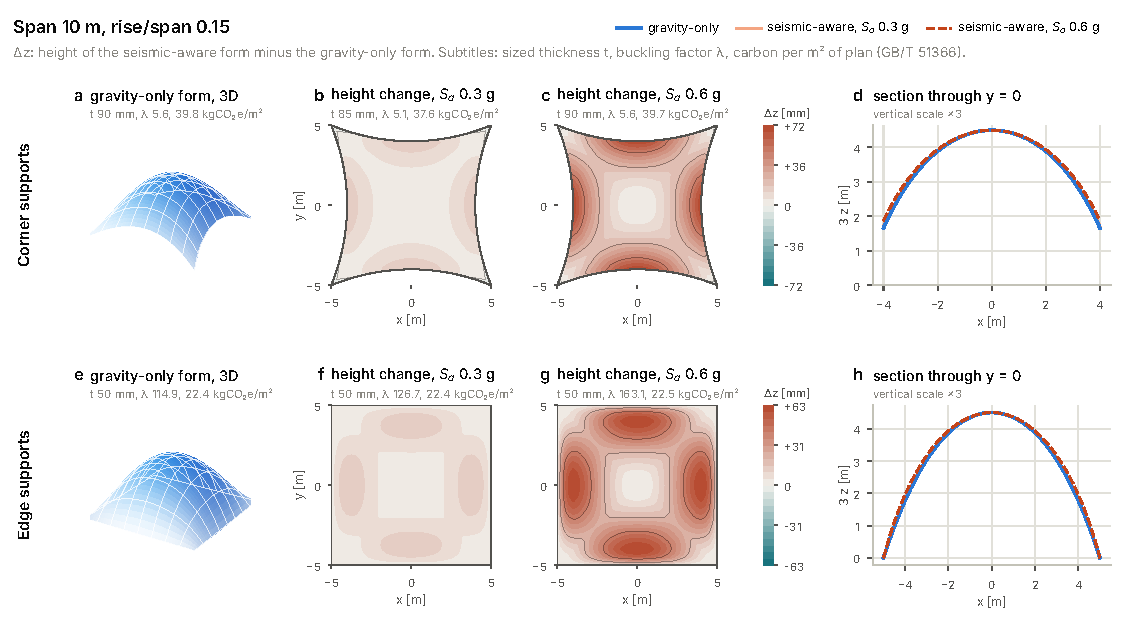
\includegraphics[width=\figwidth]{gallery_10m.pdf}\\[2mm]
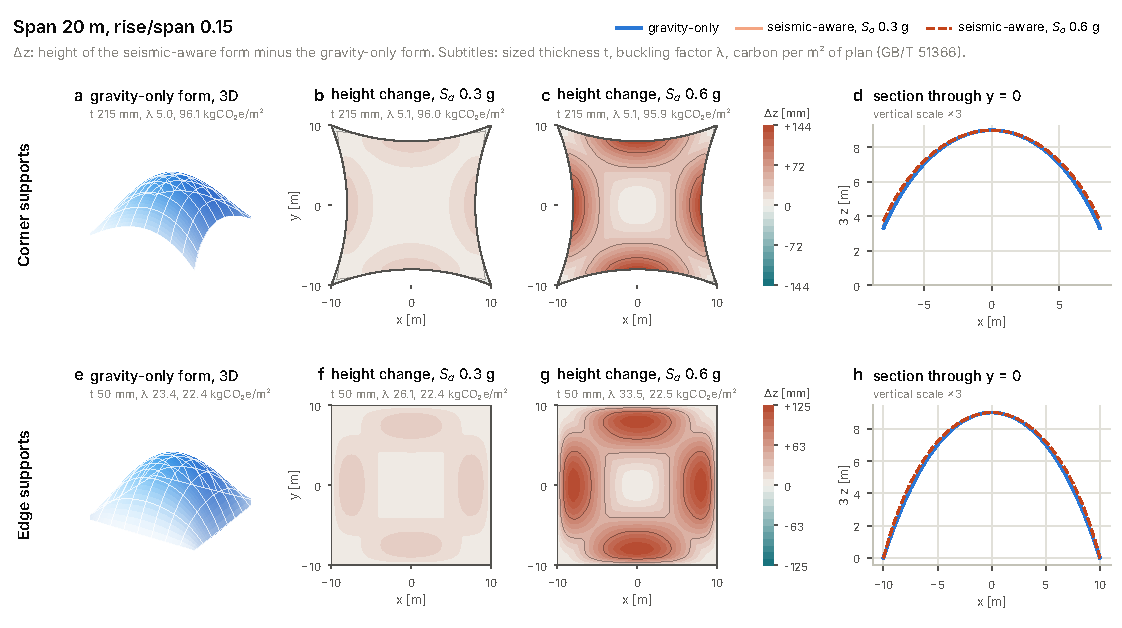
\includegraphics[width=\figwidth]{gallery_20m.pdf}
\caption{Gravity-only and seismic-aware forms at rise 0.15: (top) 10~m span, (bottom) 20~m span. In each, the rows are corner and edge supports; the panels give the gravity-only form, the height change $\Delta z$ of the seismic-aware form at $S_a$ = 0.3 and 0.6~g, and a section through $y = 0$ (vertical scale $\times$3). Panel subtitles give the sized thickness, buckling factor and carbon per m$^2$ of plan.}
\label{fig:gallery}
\end{figure}

These differences are small because the four directions of shaking cancel\jud. A form found for one direction leans: the 10~m parabolic arch of test S4, at rise-to-span 1/4, leans its crown by 0.75~m at 0.3~g. The midrange of four opposite leans keeps almost none of that lean and only lifts the surface where the four thrust surfaces spread apart. So the first question is whether the code checks see such a small change at all.

\subsection{What sets the thickness}

Fig.~\ref{fig:mechanism} shows, for all 168 designs, how close each check is to its limit at the sized thickness. One check sets the thickness in every design, and it depends only on the support condition. Linear buckling governs all 84 corner-supported designs: $\lambda_\mathrm{min}/\lambda$ is 0.888--0.997 at 10~m and 0.956--0.999 at 20~m, below 1 only because of the 5~mm thickness step. The 50~mm minimum governs all 84 edge-supported designs; their next-closest check is buckling, at 0.020--0.074 of its limit at 10~m and 0.095--0.357 at 20~m. Compression reaches at most 0.51 of $f_c$ and deflection at most 0.28 of $L/300$.

\begin{figure}[!htbp]
\centering
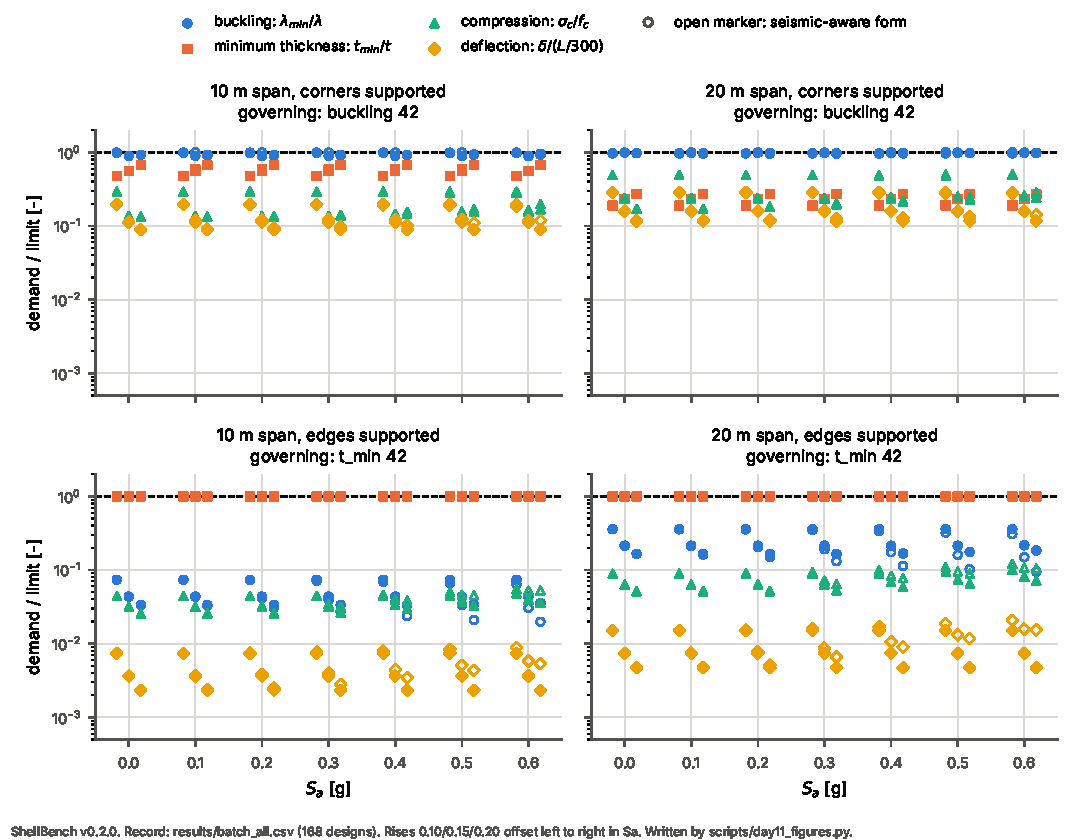
\includegraphics[width=\figwidth]{fig02_mechanism.pdf}
\caption{How close each check is to its limit at the sized thickness, for all 168 designs, by span and support condition. A ratio of 1 means the check is at its limit; the governing check is marked.}
\label{fig:mechanism}
\end{figure}

$S_a$ does not change this picture. The governing check is the same at 0~g and at 0.6~g in every design, and no other check moves onto its limit. Table~\ref{tab:sized} gives the result in thickness. Corner-supported shells need 75--105~mm at 10~m and 185--265~mm at 20~m, set by the rise; edge-supported shells stay at 50~mm everywhere.

\begin{sidewaystable}
\centering
\caption{Sized designs by span, supports and rise: ranges over both strategies and all seven $S_a$ levels (14 designs per row). Carbon at the central factors; the band corners for every design are in Table~S1.}
\label{tab:sized}
\scriptsize
\begin{tabular}{rlrrlrlllrr}
\toprule
$L$ (m) & Supports & $f/L$ & Feasible & Governs & $t$ (mm) & $\lambda$ & $T_1$ (s) & Steel (kg) & \shortstack{Carbon\\(kgCO$_2$e/m$^2$)} & \shortstack{Concrete\\share (\%)} \\
\midrule
10 & corners & 0.10 & 14/14 & buckling & 105 & 5.05--5.10 & 0.182--0.184 & 275 & 45.5 & 80.7 \\
10 & corners & 0.15 & 14/14 & buckling & 85--90 & 5.02--5.63 & 0.159--0.167 & 224--238 & 37.6--39.8 & 80.9--81.0 \\
10 & corners & 0.20 & 14/14 & buckling & 75 & 5.26--5.54 & 0.164--0.180 & 202--204 & 34.0--34.3 & 81.0--81.1 \\
10 & edges & 0.10 & 14/14 & $t_{\mathrm{min}}$ & 50 & 67.93--78.51 & 0.044--0.045 & 173 & 21.6 & 81.2 \\
10 & edges & 0.15 & 14/14 & $t_{\mathrm{min}}$ & 50 & 114.94--163.12 & 0.034--0.037 & 179--180 & 22.4--22.5 & 81.2 \\
10 & edges & 0.20 & 14/14 & $t_{\mathrm{min}}$ & 50 & 140.91--252.17 & 0.029--0.034 & 188--190 & 23.4--23.8 & 81.2 \\
20 & corners & 0.10 & 14/14 & buckling & 260--265 & 5.00--5.20 & 0.306--0.308 & 2864--2953 & 114.9--117.3 & 79.9--80.2 \\
20 & corners & 0.15 & 14/14 & buckling & 215 & 5.04--5.09 & 0.253--0.261 & 2318--2336 & 95.9--96.2 & 80.6--80.7 \\
20 & corners & 0.20 & 14/14 & buckling & 185 & 5.08--5.23 & 0.259--0.279 & 2028--2057 & 84.7--85.2 & 80.6--81.0 \\
20 & edges & 0.10 & 14/14 & $t_{\mathrm{min}}$ & 50 & 14.00--16.32 & 0.107--0.111 & 692--693 & 21.6 & 81.2 \\
20 & edges & 0.15 & 14/14 & $t_{\mathrm{min}}$ & 50 & 23.14--33.50 & 0.082--0.090 & 718--722 & 22.4--22.5 & 81.2 \\
20 & edges & 0.20 & 14/14 & $t_{\mathrm{min}}$ & 50 & 27.22--52.89 & 0.069--0.081 & 751--762 & 23.4--23.8 & 81.2 \\
\bottomrule
\end{tabular}

\end{sidewaystable}

Steel follows the same pattern. The minimum ratio governs the reinforcement almost everywhere, and the seismic case adds at most 0.82~kg of steel to a 10~m corner shell, 0.95~kg to a 20~m edge shell and 57.9~kg to a 20~m corner shell, which carries 2028--2953~kg in total. Concrete is 79.9--81.2\,\% of the carbon of every design.

This is the mechanism of the study\jud. Thickness is set by buckling or by the code minimum, steel by the minimum ratio, and none of the three responds to $S_a$ between 0 and 0.6~g. Carbon therefore has no route to depend on $S_a$, or on which form is used. The pre-registered comparison tests this directly.

\subsection{The pre-registered comparison}

Fig.~\ref{fig:difference} shows the carbon difference between the two strategies in each of the 84 cells (span, supports, rise and $S_a$), against the 5\,\% rule. In 79 of the 84 cells there is no meaningful difference. In the other 5 cells the seismic-aware form is cheaper by 5.5--5.7\,\%; all 5 are 10~m corner-supported shells at rise 0.15, $S_a$ 0.1--0.5~g. Every verdict is the same at all four corners of the $\pm$25\,\% factor band, because the band moves both strategies almost equally. The headline claim holds in 4 of its 10 scope cells at 10~m and in 0 of 10 at 20~m, so it is not made (Table~\ref{tab:verdicts}).

\begin{figure}[!htbp]
\centering
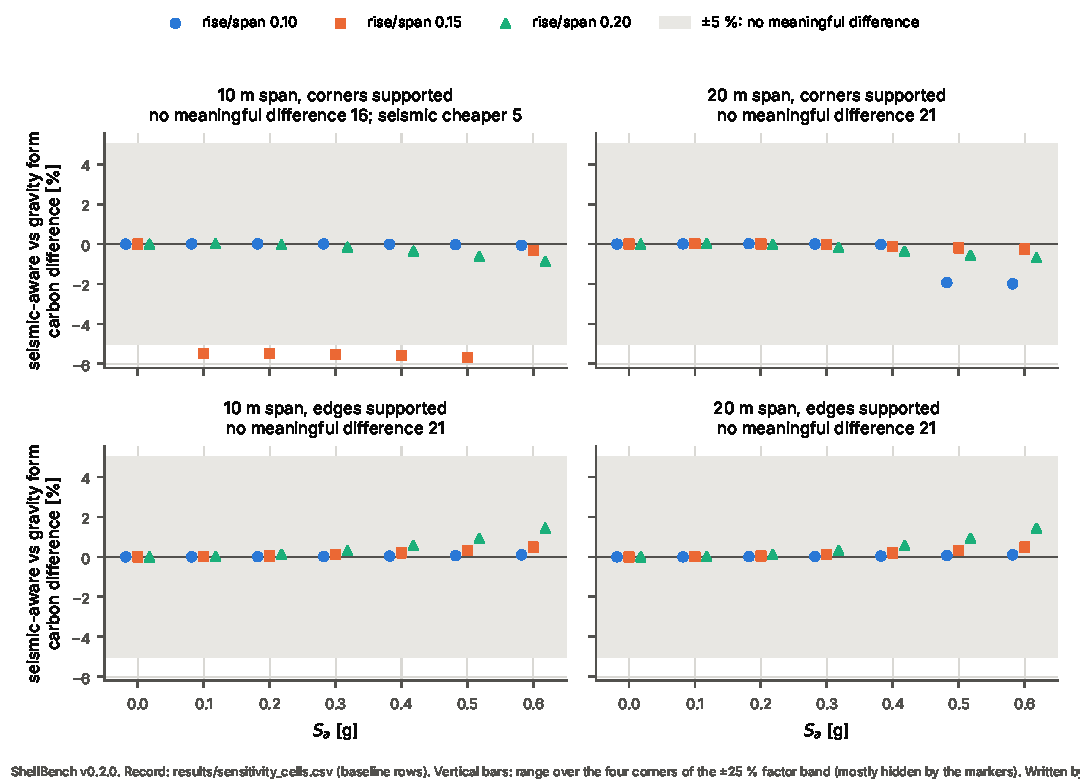
\includegraphics[width=\figwidth]{fig03_strategy_difference.pdf}
\caption{Carbon difference between the seismic-aware and the gravity-only form in each of the 84 cells, against the pre-registered 5\,\% rule, by span and support condition.}
\label{fig:difference}
\end{figure}

The 5 cells are one thickness step, not a saving\jud. At 85~mm the gravity form has $\lambda = 4.978$ and fails by 0.4\,\%, while the seismic-aware forms at 0.1--0.5~g have $\lambda = 5.016$--5.052 and pass by at most 1.0\,\%. So the seismic-aware shells size to 85~mm and the gravity shells to 90~mm. Each of the three sensitivity runs removes them: the $61 \times 61$ network and either buckling threshold (Section~\ref{sec:drivers}). In each case both strategies size to the same thickness. We report the 5 cells as a grid-step artefact.

So the comparison confirms the mechanism. The next question is how large the effect of $S_a$ is next to the other choices a designer makes.

\subsection{What moves carbon}\label{sec:drivers}

Fig.~\ref{fig:drivers} puts every driver of carbon on one scale. For the gravity-only form, raising $S_a$ from 0 to 0.6~g changes carbon by at most 0.4\,\%. For the seismic-aware form the change is $-5.7$ to $+1.5$\,\%, and the strategy itself moves carbon by $-5.7$ to $+1.4$\,\%; the extreme values are the 5 artefact cells. The buckling threshold moves much more. For the gravity-only corner shells at $S_a = 0$, carbon falls to 0.736--0.812 of the baseline at $\lambda \geq 3$ and rises to 1.220--1.295 at $\lambda \geq 8$; over all 84 corner designs the ranges are 0.732--0.826 and 1.219--1.295 (Fig.~\ref{fig:drivers}). For the 10~m corner shell at rise 0.15, for example, the thickness is 70, 90 and 110~mm at $\lambda \geq 3$, 5 and 8, and its carbon is 31.1, 39.8 and 48.6~kgCO$_2$e/m$^2$. The buckling threshold, a choice that no code fixes for shells, therefore moves corner-shell carbon by 19--29\,\%, an order of magnitude more than the seismic level up to 0.6~g\jud. Edge-supported shells respond to nothing except the factor band, because they sit on the code minimum.

\begin{figure}[!htbp]
\centering
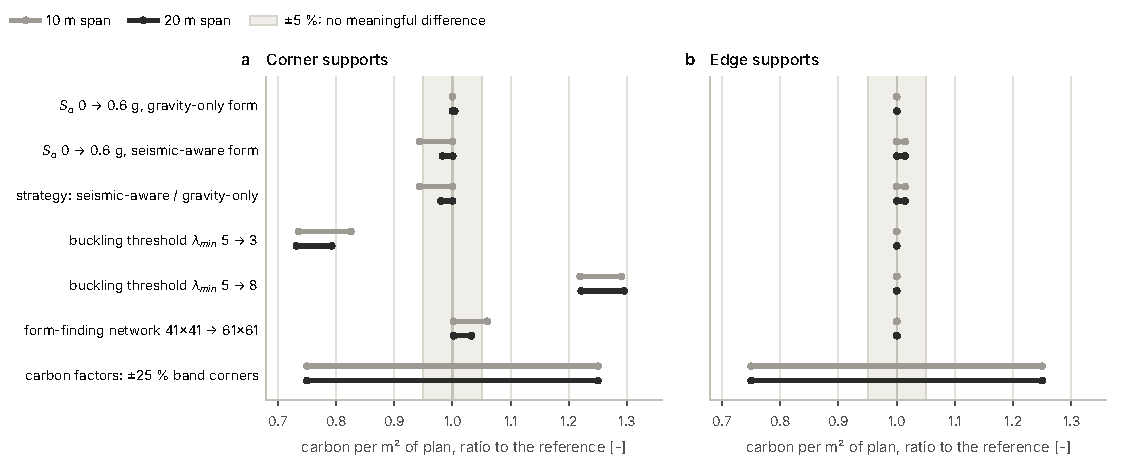
\includegraphics[width=\figwidth]{fig04_carbon_drivers.pdf}
\caption{What moves carbon. Each bar is the range, over all designs of a span and support condition, of the carbon per m$^2$ of plan as a ratio to its reference: the same design at $S_a = 0$, the gravity-only form, or the baseline settings ($\lambda \geq 5$, $41 \times 41$, central factors). The shaded band is the 5\,\% rule.}
\label{fig:drivers}
\end{figure}

The verdicts barely move under the three sensitivity runs (Table~\ref{tab:verdicts}). At 20~m every cell is no meaningful difference in all three runs. At 10~m, $\lambda \geq 8$ and the $61 \times 61$ network give no meaningful difference in all 42 cells. $\lambda \geq 3$ gives 40 cells of no meaningful difference and 2 of ``gravity cheaper'', and these 2 need their own explanation. In every run, every verdict is the same at all four band corners, and the headline holds in 0 of 10 scope cells at both spans.

\begin{sidewaystable}
\centering
\caption{Pre-registered comparison under the baseline and the three sensitivity runs. A difference below 5\,\% is no meaningful difference. ``$t$ changed'': designs whose thickness differs from the baseline. Headline scope: rise 0.15, both supports, $S_a \geq 0.2$~g (10 cells per span).}
\label{tab:verdicts}
\scriptsize
\begin{tabular}{>{\raggedright\arraybackslash}p{0.17\linewidth}rrr>{\raggedright\arraybackslash}p{0.22\linewidth}rrrr}
\toprule
Run & $L$ (m) & Feasible & \shortstack{$t$\\changed} & Verdicts (central factors) & \shortstack{Same at all\\4 corners} & \shortstack{Largest\\$|\Delta|$ (\%)} & \shortstack{Headline\\cells} & \shortstack{Headline\\made} \\
\midrule
baseline ($\lambda$ $\geq$ 5, 41 $\times$ 41) & 10 & 84/84 & 0 & no meaningful difference 37; seismic cheaper 5 & 42/42 & 5.7 & 4/10 & no \\
baseline ($\lambda$ $\geq$ 5, 41 $\times$ 41) & 20 & 84/84 & 0 & no meaningful difference 42 & 42/42 & 2.0 & 0/10 & no \\
$\lambda$ $\geq$ 3 & 10 & 84/84 & 42 & gravity cheaper 2; no meaningful difference 40 & 42/42 & 8.4 & 0/10 & no \\
$\lambda$ $\geq$ 3 & 20 & 84/84 & 42 & no meaningful difference 42 & 42/42 & 3.6 & 0/10 & no \\
$\lambda$ $\geq$ 8 & 10 & 84/84 & 42 & no meaningful difference 42 & 42/42 & 1.4 & 0/10 & no \\
$\lambda$ $\geq$ 8 & 20 & 84/84 & 42 & no meaningful difference 42 & 42/42 & 2.5 & 0/10 & no \\
61 $\times$ 61 network & 10 & 84/84 & 5 & no meaningful difference 42 & 42/42 & 1.5 & 0/10 & no \\
61 $\times$ 61 network & 20 & 84/84 & 12 & no meaningful difference 42 & 42/42 & 2.6 & 0/10 & no \\
\bottomrule
\end{tabular}

\end{sidewaystable}

The 2 new cells are the same grid step pointing the other way. They are 10~m corner shells at rise 0.20 and $S_a$ 0.5 and 0.6~g. At 55~mm the gravity form has $\lambda = 3.0003$ and passes by 0.01\,\%. The seismic-aware forms have $\lambda = 2.936$ and 2.846 and fail, so they size to 60~mm and carry 8.4\,\% and 8.2\,\% more carbon. At equal thickness the seismic-aware form buckles at a 2--5\,\% lower load here, and one 5~mm step (9\,\% of 55~mm) turns that into an 8\,\% carbon difference. Near a threshold, which strategy ``wins'' depends only on which side of a thickness step each form falls\jud. The 5\,\% rule cannot separate differences smaller than one step on shells this thin.

The $61 \times 61$ network changes little. All 168 designs remain feasible, and 17 of 168 thicknesses move by one 5~mm step (5 at 10~m, 12 at 20~m). At equal thickness the corner buckling factor moves by at most 2.0\,\%. Gravity-form carbon at $S_a = 0$ is 1.000--1.026 of the $41 \times 41$ value. The 5 baseline ``seismic cheaper'' cells vanish here as well. So the result does not depend on the buckling threshold, the network or the factor band. It does rest on the equivalent static load, which the next section checks.

\subsection{The equivalent static load is on the safe side}

Fig.~\ref{fig:periods} places the first period of every baseline design on the GB 50011 design spectrum shape read from ShellBench. All 168 designs have $T_1$ between 0.029 and 0.308~s, at or below $T_g = 0.35$~s, so test S5 has no failure; the same holds in all three sensitivity runs (longest $T_1$ 0.341~s, at $\lambda \geq 3$). The corner-supported shells sit on the plateau. 70 of the 84 edge-supported designs are stiffer still and sit on the rising branch, where the spectral value is 0.61--0.95 of the plateau value. For them the plateau load we used is conservative\jud. The no-difference result is therefore not caused by an underestimated seismic load. Its limits lie elsewhere: linear buckling without imperfections, and an equivalent static load in place of a dynamic analysis. Section~\ref{sec:discussion} discusses both.

\begin{figure}[!htbp]
\centering
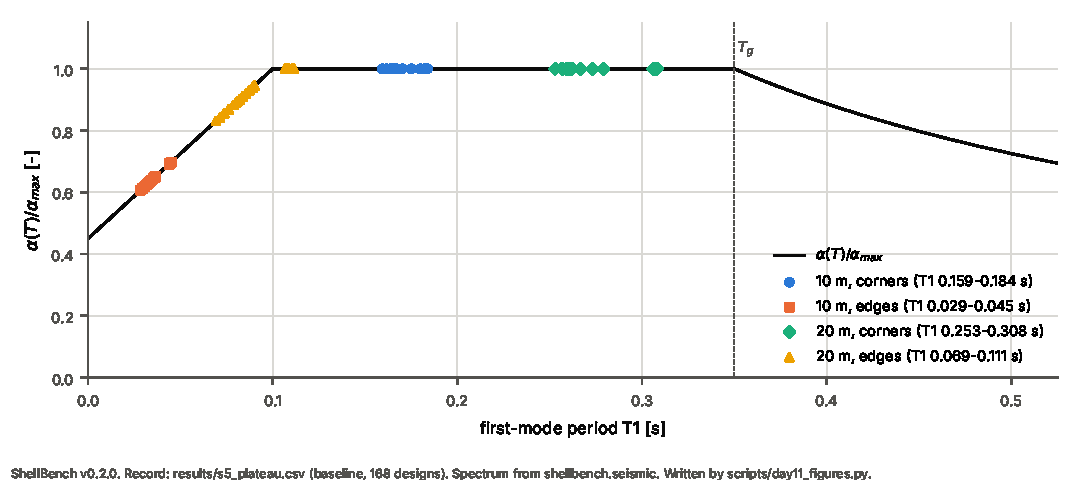
\includegraphics[width=\figwidth]{fig05_s5_periods.pdf}
\caption{First periods of all 168 baseline designs on the normalised GB 50011 design spectrum read from ShellBench ($T_g = 0.35$~s), by span and support condition.}
\label{fig:periods}
\end{figure}

\subsection{Verification of the analysis chain}\label{sec:verification}

The checks in this section were added after the freeze. They test the tools, not the hypothesis, and none of them changes a thickness or a verdict (Fig.~S1).

The buckling path matches the classical value on a sphere. A complete sphere under external pressure, meshed with the same S8R elements and solved with the same eigenvalue step, buckles at 1.96\,\% above the classical value at $R/t = 50$ and 1.33\,\% above it at $R/t = 100$, on the finest of five meshes (3456 elements). The offset falls with $t/R$ and matches the membrane stiffness of the same model, which is 1.49\,\% and 0.75\,\% too stiff. We read it as the thickness effect of the solid-element expansion of S8R, not as a mesh error\jud. The sized shells are thinner than either sphere ($R/t$ of about 78 to 520), so we did not test their whole range.

The record network is fine enough for buckling but not for deflection at a point support. On eight designs refined from 21 to 81 nodes per side at their frozen thickness, $\lambda_1$ changes by at most 0.62\,\% between the two finest networks. On the record network ($41 \times 41$) the corner-shell $\lambda_1$ is above the finest value by 0.8--1.0\,\% for the gravity-only form and 1.6\,\% for the seismic-aware form. This is the bias that the $61 \times 61$ sensitivity run already measured, and it removed only the 5 grid-step cells (Section~\ref{sec:drivers}). The edge-supported shells, far above their limit, read up to 5.8\,\% high. The SLS deflection of corner-supported shells does not converge: it grows by 3.8--5.8\,\% per refinement, because its largest value sits next to a point support. It never comes near the limit. On the finest network the largest deflection is 0.18 of $L/300$.

The form-finding is in equilibrium to round-off. The residual of the assembled force density system is below $2.5 \times 10^{-11}$~N for unit nodal weights, over all 84 solves (four families, three rises, seven $S_a$ levels), on both machines that ran the check.

The shells carry the design lateral load mainly as membranes. Membrane action holds 76.3--89.2\,\% of the strain energy of the corner-supported shells and 91.0--99.9\,\% of the edge-supported ones, over all 168 designs and both ULS cases. The seismic-aware form has the smaller share in every one of the 72 cells with $S_a > 0$, under both cases, by up to 13 percentage points; the lateral case itself lowers the share in 129 of the 144 designs with $S_a > 0$, by at most 2.8 points. For the 10~m shells at rise 0.15 and $S_a = 0.6$~g under the seismic case, the share is 87.3\,\% (gravity-only) and 84.3\,\% (seismic-aware) with corner supports, and 97.6\,\% and 94.3\,\% with edge supports. We read this as the price of one form for four directions of shaking: it is funicular for none of them\jud.

Formwork cannot turn a ``no meaningful difference'' verdict into a difference. Its carbon scales with the soffit area, and the soffit areas of the two strategies differ by at most 1.44\,\% in any cell. Adding a formwork term of any size to both strategies gives a difference that lies between the carbon difference and the area difference. So, whatever the formwork factor and whether the formwork is used once, 5 times or 20 times, the 79 ``no meaningful difference'' cells stay inside the 5\,\% band. The absolute carbon would change; ShellBench holds no formwork factor yet, so we give none.

Fig.~\ref{fig:pareto} puts carbon against $\lambda_1$ for every sized design. The non-dominated front is made only of edge-supported shells: they sit on the 50~mm minimum with $\lambda_1$ of 68--252 (10~m) and 14--53 (20~m) at 21.6--23.8~kgCO$_2$e/m$^2$. Corner-supported shells sit on the threshold they were sized to, and each step from $\lambda \geq 3$ to 5 to 8 costs carbon. The two strategies lie on top of each other. The support condition and the buckling threshold move the trade-off between stability and carbon; the strategy does not.

\begin{figure}[!htbp]
\centering
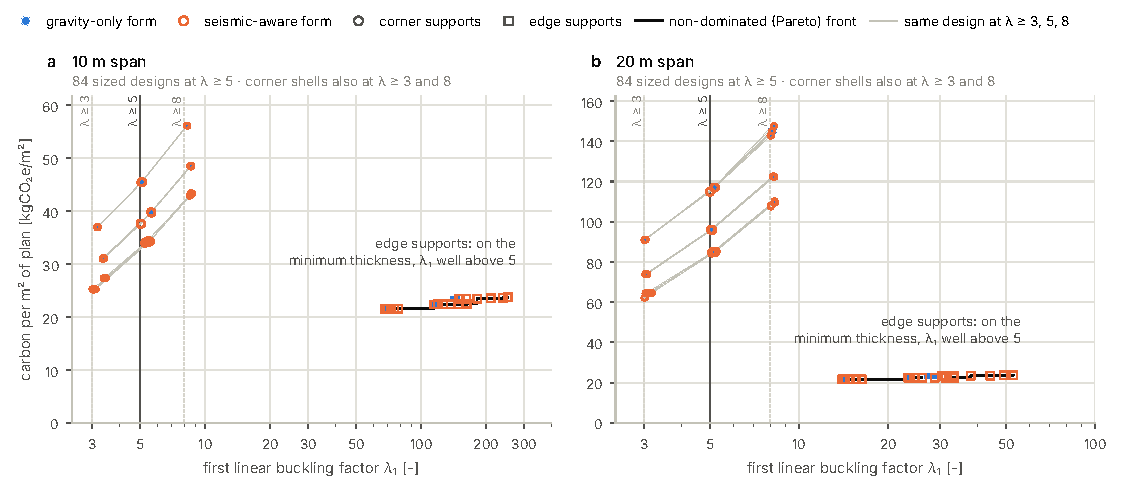
\includegraphics[width=\figwidth]{fig06_carbon_stability.pdf}
\caption{Carbon per m$^2$ of plan against the first buckling factor $\lambda_1$ for every sized design at $\lambda \geq 3$, 5 and 8, for 10 and 20~m spans, with the non-dominated (Pareto) front.}
\label{fig:pareto}
\end{figure}

%% ---------------------------------------------------------------------
\section{Discussion}\label{sec:discussion}

\subsection{Why the seismic level does not reach the carbon}

The result is a null, and it has a cause. In every one of the 168 designs, the thickness is set by linear buckling or by the 50~mm minimum, and the steel by the minimum ratio (Section~3.2). None of the three responds to the seismic level between 0 and 0.6~g. So carbon cannot follow $S_a$, and it cannot follow the form either, because the two forms differ by at most 0.7\,\% of the span (Section~3.1).

This holds for reinforced concrete shells of 10 and 20~m, square in plan, on corner or edge supports, sized to code checks under an equivalent static load. It does not hold, as far as we know, for shells whose material has no tensile capacity. There the form itself must keep the thrust inside the section, and a lateral load can make a gravity form infeasible; that is the setting in which Michiels and Adriaenssens developed seismic form-finding \cite{Michiels2017IASS,Michiels2018CS}\chk. Reinforcement takes that job away from the form. The minimum steel ratio, which every shell carries anyway, covers the tension that the small lateral load adds\jud.

A second reason is the four directions of shaking. A form found for one direction leans, as the S4 arch does (0.75~m at the crown at 0.3~g, Section~3.1). A form that must serve four opposite directions keeps the midrange of four leans, which keeps almost none of the lean. The seismic-aware strategy therefore converges back towards the gravity form. We see this as a property of the strategy, not of our code: any form that must carry reversing lateral load with one surface meets the same cancellation\jud.

\subsection{The strongest objection, and our answer}

The strongest objection is that the comparison was set up so that it could not find a difference. If the seismic-aware form can only rise and never lean, and if linear buckling governs, then perhaps the study tested a weak strategy against a check that cannot see it.

We take this in two parts. First, the strategy. We used the method Michiels and Adriaenssens proposed for lateral load, extended to four directions and to a three-dimensional network, and we checked our lateral-load code against the closed-form leaned parabola within the pre-registered tolerance of $10^{-9}$ (test S4). A one-direction form would lean more, but it would fail when the shaking reverses, so it is not a design option for a building. Second, the check. Linear buckling does respond to the form: at equal thickness, the seismic-aware form buckles at a 2--5\,\% lower load in the cells near $\lambda \geq 3$ (Section~\ref{sec:drivers}). The check sees the form; the form is simply too close to the gravity form for the difference to cross one 5~mm thickness step in most cells. Where it does cross, the sign is not consistent. At $\lambda \geq 5$, five cells favour the seismic-aware form, and at $\lambda \geq 3$ two cells favour the gravity form. Both are the same step effect pointing in opposite directions.

So the null is not built into the design of the study\jud. A shell that the code checks pushed close to the boundary between two thickness steps would show a difference, and in a few cells it does. What the study shows is that such differences are smaller than the resolution of practical sizing, and that their sign depends on where the step falls, not on the strategy.

\subsection{What does move carbon}

For these shells the carbon is set by the support condition and by the buckling factor a designer chooses. Corner-supported shells carry 75--105~mm at 10~m and 185--265~mm at 20~m, edge-supported shells 50~mm everywhere (Table~\ref{tab:sized}). Moving the buckling threshold from 5 to 3 or 8 moves corner-shell carbon by 19--29\,\%, against at most 0.4\,\% for the seismic level on the gravity form (Section~\ref{sec:drivers}).

This matters more than the null itself\jud. No code fixes the buckling factor for shells: ACI 318.2-14 requires only that instability be ``precluded'' \cite[cl.~3.1.8]{ACI3182}, and the reduction-factor approach \cite{Dulacska1995} leaves the reductions for imperfection, creep and cracking to the designer. Read through that approach, our three thresholds correspond to combined reductions of 1.0, 0.6 and 0.375 under a safety factor of 3.0 (Section~\ref{sec:checks}). The carbon of a corner-supported concrete shell therefore depends on an engineering judgement that is rarely reported. A study that compares shell forms, or shells against other roofs, should report its buckling factor and its sensitivity, as we do in Table~\ref{tab:verdicts}.

For edge-supported shells the answer is simpler. They sit at the 50~mm minimum with a buckling factor far above any threshold (Section~3.2). Their carbon is set by the constructible minimum, so a lower minimum, for example from a thinner mesh layout or a different cover rule, would lower their carbon directly, and a different form would not.

\subsection{What this means for design}

For a designer of a reinforced concrete shell roof in the range studied, the message is practical. Form-find for gravity. Then check the seismic combinations. Sized to the same checks, the gravity form was feasible in all 84 of its designs, at a cost of resilience of 1.000--1.004 up to 0.6~g. Spend the design effort on the support condition, the buckling factor and the minimum thickness, because these set the carbon.

The method is the part that transfers beyond shells\jud. The study pre-registered its rules before any run, sized every design to the same code checks, compared strategies with a fixed decision rule, and asked which check governs before asking which form wins. That sequence separates a real carbon saving from a sizing artefact, and it applies to any structure in which a design strategy is meant to save material: the saving is real only if it changes the governing check.

\subsection{Limitations}

We state each limit with what would remove it.

\textit{Linear buckling without imperfections.} Buckling governs every corner shell, and we used the linear factor with a safety threshold in place of a geometrically nonlinear analysis with imperfections. An imperfection-sensitive analysis could separate the two forms more than the linear factor does, because the seismic-aware form changes the curvature near the edges. A nonlinear buckling analysis of the governing cells, with an imperfection of 1/4 to 3/4 of the thickness as Dul\'acska and Koll\'ar suggest \cite[p.~317]{Dulacska1995}, would test this. The linear factor itself is accurate where we could check it: on a sphere it lies within 2\,\% of the classical value, and it is mesh-converged to 0.6\,\% (Section~\ref{sec:verification}).

\textit{Equivalent static load.} We applied the plateau spectral value as a uniform lateral acceleration. Every first period lies at or below $T_g$, so the load is on the plateau or conservative (Section~3.5), but higher modes and vertical excitation were not modelled. A response-spectrum or time-history analysis of the governing cells would remove this limit.

\textit{One material, one plan, two spans.} Reinforced concrete C40, square plans, 10 and 20~m. Longer spans, heavier finishes and unreinforced shells are where we expect the null to break (Section~4.1). The code is open, so each of these is one change to the design space.

\textit{Uniform thickness and net steel.} Each shell has one thickness, and steel is a net take-off without laps or waste. Both apply to both strategies alike, so they do not affect the comparison, but they affect the absolute carbon.

\textit{A1--A3 only, one factor source.} Carbon covers product stages A1--A3 with GB/T 51366 factors and a $\pm$25\,\% band. Every verdict holds at all four corners of the band, so the comparison does not depend on the factors; the absolute values do. Formwork is outside the boundary. It cannot change the comparison, because the soffit areas of the two strategies differ by at most 1.44\,\% (Section~\ref{sec:verification}), but it would raise the absolute carbon by an amount that depends on its factor and its number of uses.

\textit{The buckling threshold is a judgement.} We could not read the IASS (1979) recommendations, and neither source we read states the factor of 5. We therefore report it as an assumption and give the full study at 3 and 8 (Section~\ref{sec:checks}, Table~\ref{tab:verdicts}).

%% ---------------------------------------------------------------------
\section{Conclusions}\label{sec:conclusions}

This study asked whether seismic-aware form-finding lowers the embodied carbon of reinforced concrete shells sized to code checks. For square shells of 10 and 20~m, on corner or edge supports, up to a plateau spectral acceleration of 0.6~g, it does not. Four conclusions follow.

\begin{enumerate}
\item The two strategies give the same carbon. In 79 of 84 pre-registered comparisons they differ by less than 5\,\%. The other 5 are one 5~mm thickness step, and they disappear under each of the three sensitivity runs. The headline claim, that the seismic-aware form is cheaper, is not made.
\item The governing checks explain why. Linear buckling sets the thickness of every corner-supported shell, the 50~mm minimum sets every edge-supported shell, and the minimum steel ratio sets the reinforcement. None of the three responds to the seismic level. The seismic case adds at most 57.9~kg of steel to a 20~m corner shell that carries 2028--2953~kg.
\item The buckling factor moves carbon; the seismic level does not. Changing the buckling threshold from 5 to 3 or 8 gives gravity-form corner-shell carbon of 0.736--0.812 or 1.220--1.295 of the baseline. Raising the seismic level from 0 to 0.6~g changes gravity-form carbon by a factor of 1.000--1.004. Since no code fixes the buckling factor for shells, studies of shell carbon should report it and its sensitivity.
\item The equivalent static load is on the safe side. Every first period is at or below $T_g = 0.35$~s, so the shells sit on the plateau or on the rising branch of the spectrum.
\end{enumerate}

For design in this range, form-find for gravity, check the seismic combinations, and spend the effort on the support condition, the buckling factor and the minimum thickness\jud. The result should change where the form must keep the thrust inside the section, as in unreinforced shells, and may change for longer spans, heavier roofs, imperfection-sensitive buckling or a dynamic analysis. Each is one change to the open pipeline. The pipeline itself, with pre-registered rules, the same code checks for every design, and the question of which check governs asked before the question of which form wins, applies to any design strategy that claims to save material\jud.

%% ---------------------------------------------------------------------
\section*{CRediT authorship contribution statement}

\textbf{Syed Nafiz Reja Hasib:} Conceptualization, Methodology, Software, Validation, Formal analysis, Investigation, Data curation, Visualization, Writing -- original draft, Writing -- review \& editing.\chk

\section*{Declaration of competing interest}

The author declares no known competing financial interests or personal relationships that could have appeared to influence the work reported in this paper.\chk

\section*{Funding}

This research did not receive any specific grant from funding agencies in the public, commercial or not-for-profit sectors.\chk

\section*{Data and code availability}

The code, the frozen results of all 168 designs, the sensitivity runs and the scripts that build every figure and table are openly available as ShellForm v0.1.0 at \url{https://doi.org/10.5281/zenodo.24084111} (all versions: \url{https://doi.org/10.5281/zenodo.24084110}) and at \url{https://github.com/syednafizreja/ShellForm}; the frozen run is git tag \texttt{freeze-2026-11-09}. The verification add-ons of Section~\ref{sec:verification} were run after that release and are on the repository's main branch; they will be archived in the next release \unk. Every input value is read from ShellBench v0.3.0 (git tag \texttt{v0.3.0}; archive \url{https://doi.org/10.5281/zenodo.23851675}) \cite{ShellBench}. Code clauses are cited by number; the standards themselves are not redistributed.

\section*{Declaration of generative AI and AI-assisted technologies in the writing process}

During the preparation of this work the author used Claude (Anthropic) to draft and edit the text from the author's results, notes and rules, to write and review analysis code, and to check numbers against the result files. After using this tool, the author reviewed and edited the content as needed and takes full responsibility for the content of the publication.\chk

\bibliographystyle{elsarticle-num}
\bibliography{references}

\end{document}
